\chapter{Memorias}
\label{cap:memorias}

La memoria es un acto en el presente. En tal acto, tanto la imaginación como las experiencias, las competencias, las necesidades, los intereses, las emociones, los sentimientos y los sesgos personales no pueden no influir. Las expectativas personales y sociales también pesan en el presente acto de recordar. \emph{Recordar} es volver a pasar por el corazón, \emph{recordar} es volver a sonar. Con esto en mente, con la conciencia de que recordar es un acto creativo, intento traer a mi memoria tanto la primer reunión con las autoridades universitarias como la reunión entre «Pajarito», Juan Martín y yo.


\section{El canto y las palabras de un hijo}
\label{sec:palabra-canto}

\begin{figure}[H]
\centering
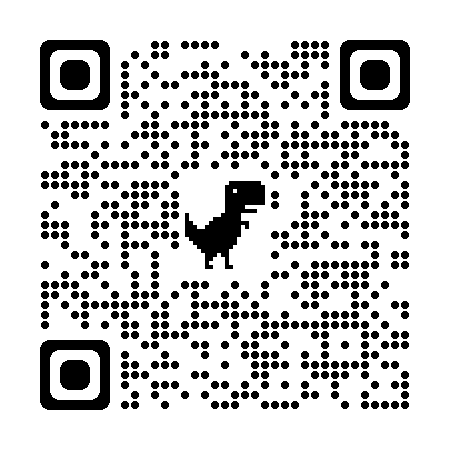
\includegraphics[width=0.3\textwidth]{img/qrcode-himno-memoria}
\caption[El canto y las palabras de \textsc{Juan Martín Leguizamón}]{El canto y las palabras de \textsc{Juan Martín Leguizamón}. URL: \url{https://drive.google.com/drive/folders/1ynZQ9jA4grgtdlFFCoR9SALISPsIrsq_}}
\label{fig:canto-palabras}
\end{figure}


En diciembre de 2022 me contacta \textsc{Marcelo «Pajarito» Sutti}\footnote{\textsc{Marcelo Sutti} es destacado poeta y músico salteño.}, quien me informa que \textsc{Juan Martín Leguizamón}\footnote{\textsc{Juan Martín Leguizamón}, hijo de Gustavo, es antropólogo y presidente de la Fundación Legado Cultural Cuchi Leguizamón.} le refiere tener viva en su memoria una melodía que recuerda bajo el título de \emph{Himno a la UNSa}. Enteradas las autoridades de la Universidad del relato de Juan Martín ---y mediado por Sutti quien me señala ante ellas como un hombre idóneo para realizar un peritaje sobre la melodía en memoria del hijo del «Cuchi»---, organizan una reunión en la que acordamos trabajar sobre el fragmento recordado y su posible relación con los modos de componer del legendario músico salteño. La posibilidad de establecer un grado de compatibilidad entre la melodía a estudiar y las melodías de Gustavo Leguizamón existe porque existen técnicas de análisis que pueden develar estructuras que muestran estilo y compatibilidad de escritura en diversas piezas de un mismo autor. El \emph{análisis schenkeriano} en este particular caso me pareció una herramienta adecuada por ser capaz de mostrar estructuras intermedias y de superficie propias de un autor específico, y es la que en esa reunión ---y en la propuesta escrita presentada a la Universidad en febrero de 2023--- propuse utilizar para la pericia.

No recuerdo si primero fue la reunión con las autoridades universitarias, o si antes fue la reunión con Sutti y Leguizamón (h). No importa\footnote{La reunión con Sutti y Leguizamón (h) fue el 20 de diciembre de 2022 en mi domicilio particular y la grabación (Figura~\ref{fig:canto-palabras}, página~\pageref{fig:canto-palabras}) fue registrada a las 16:46 horas; con las autoridades nos reunimos el día 27 del mismo mes a las 16:00 horas en un bar del centro de la ciudad de Salta.}. Sí importa que fue una tarde de verano con un cielo tapado de amenazantes y negras nubes. El momento central de esa amena y nada amenazante charla no es necesario recordarlo: el registro electrónico nos exime del acto creativo de recordar, y él es accesible con el código QR de la Figura~\ref{fig:canto-palabras}.

\begin{figure}[htb]
\begin{ly}
\relative {
  \clef "treble"
  \key es \major
  \time 12/8
  \tempo 4.= 55
  \partial 8
  bes8
  es4. ~ es4 es8 es4 c8 ~ c d es
  f4. ~ f8 f es d4. r4 bes8
  g'4. ~ g4 g8 g4 es8 ~ es f g
  aes4. aes8 aes g f4. r4 bes8
  es4. ~ es4 es8 es4 c8 ~ c d es
  d4. ~ d8 bes g bes4. r
  c8 aes4 ~ aes aes8 aes f4 ~ f8 g aes
  g4. ~ g4 g8 g4 es8 ~ es f g
  f4. ~ f8 g f c4 d bes
  es4.
}
\end{ly}
\caption[Transcripción de un fragmento de la melodía recordada.]{Transcripción de un fragmento de la melodía recordada y cantada por \textsc{Juan Martín Leguizamón.}}
\label{fig:Transcripcion}
\end{figure}

Basta con transcribir un fragmento de lo cantado por el hijo del «Cuchi» para detectar una serie de significativas características, algunas que acercan esta versión a la versión escrita (mostrada y estudiada en el Capítulo~\ref{cap:partitura}), otras que producen la divergencia entre ellas.

La tonalidad de Mi\bemoltxt\ mayor utilizada por Juan Martín ---a diferencia de la de Fa mayor consignada en la partitura--- es debido a que para su registro de voz ---y no sólo para el de él, sino para el registro vocal de la mayoría de la población--- esta tonalidad es más conveniente. La melodía escrita por su padre, en Fa mayor, es de difícil canto para la mayoría de la etnia de Salta. Sin embargo, en amplio pasaje las dos versiones coinciden en su conformación interválica, reconociéndose en la versión de Juan Martín la pieza de Gustavo Leguizamón. A tal punto es así que el 23 de abril de 2023 a la tarde, consultado yo telefónicamente por \textsc{Lucrecia Coscio}\footnote{Coordinadora del Centro Cultural Holver Martínez Borelli de la UNSa.} acerca de si algunas de las partituras que me enviaba vía \emph{WhatsApp} tenía relación con la melodía referida por Juan Martín.

\begin{figure}[H]
\centering
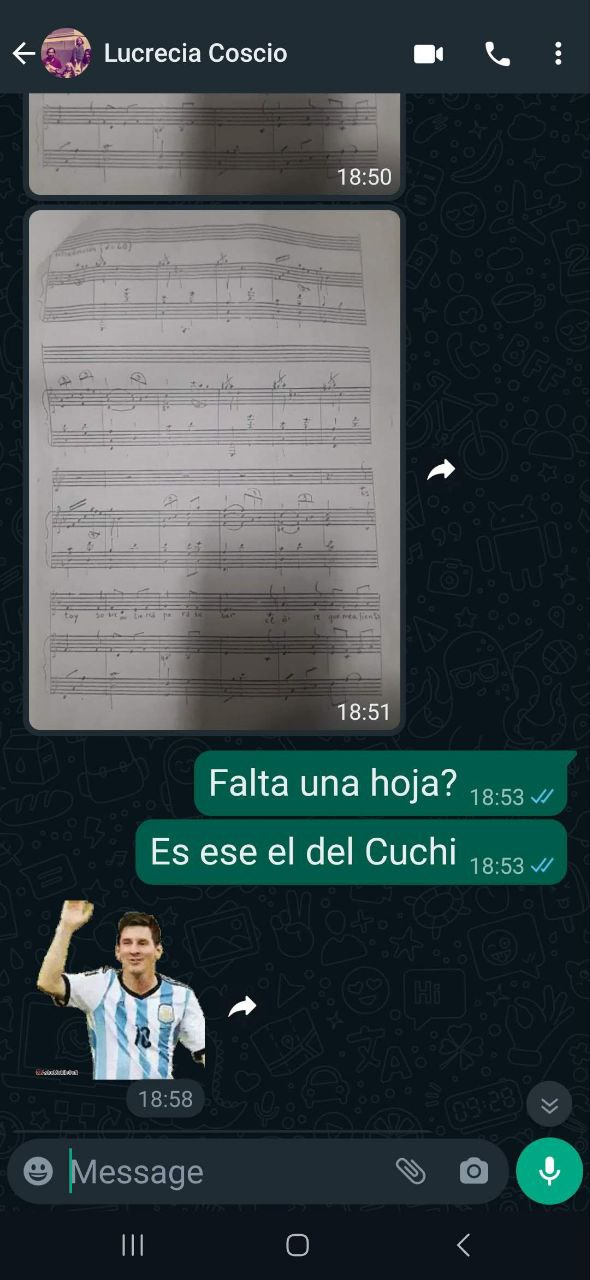
\includegraphics[width=0.3\textwidth]{img/lucrecia1}
\caption{21 de abril: hallazgo de la partitura.}
\label{fig:hallazgo-partitura}
\end{figure}

\noindent Ese mismo día, en horas de la mañana, la profesora Coscio me había enviado otras partituras que indudablemente no tenían relación con la melodía en cuestión, y así lo hice saber. Pero faltando 12 minutos para las 19:00 horas, Lucrecia vuelve a comunicarse conmigo. Mientras me dirijo a la presentación de la flamante \emph{Fundación Legado Cultural Cuchi Leguizamón} veo las fotos y reconozco de inmediato el parentesco de lo que está escrito con lo cantado durante una tormenta de verano cuatro meses atrás: es el himno del «Cuchi»\footnote{Esa misma tarde, junto a la partitura se halló un sobre conteniendo los datos de los autores de la letra y la música (ver Figura~\ref{fig:sobre-letra} en la página~\pageref{fig:sobre-letra}).}. Gol.


\section{La memoria oral y la memoria escrita}
\label{sec:memoria-oral-escrita}

En la escritura musical la representación de las alturas de los sonidos no reviste ambigüedad alguna debido a que el sistema musical convencional ---el usado por Leguizamón--- consiste en doce notas afinadas en el temperamento igual, representadas gráficamente con cabezas de notas ubicadas más arriba o más abajo sobre un pentagrama que es presidido por una clave que indica registro agudo (clave de sol), medio (claves de do) o grave (clave de fa). La representación del ritmo, basada en figuras organizadas en sistema binario\footnote{Al ser una \blanca\ la representación de una duración que es la mitad de una \redonda, la \negra\ la mitad de una \blanca, la \corchea\ la mitad de una \negra, la \semicorchea\ la mitad de una \corchea, etc., queda evidenciado que el sistema utilizado para la representación de duraciones es \emph{binario}.}, tiene limitaciones respecto a la flexibilidad con la que los seres humanos solemos tratar, a la hora de la interpretación, al ritmo musical. Sin embargo, la representación rítmica en una partitura bien escrita acerca, y mucho, la idea rítmica que un compositor tiene \emph{in mente} o en su propia experiencia interpretativa de una obra. Dicho de otro modo: si se ejecuta una partitura rígidamente, matemáticamente, se puede percibir esa interpretación como algo «deshumanizada», pero nunca muy lejos de la idea rítmica que el compositor tuvo al anotarla.

\begin{figure}[htb]
\begin{ly}
\relative {
  \key es \major
  \time 2/4
  \partial 8
  bes8
  es4. es8
  es c d es
  f4 f8 es
  d4. bes8
  g'4. g8
  g es f g
  aes4 aes8 g
  f4. bes8
  es4. es8
  es c d es
  d4 bes8 g
  bes4. c8
  aes4 aes
  aes4. bes8
  g f g es
  f c d bes
  es4.
}
\end{ly}
\caption{Fragmento de la partitura del \emph{Himno} transportado a Mi\bemoltxt\ mayor.}
\label{fig:frag-partitura}
\end{figure}

Volvamos por unos instantes al fragmento transcripto de la versión oral de Juan Martín Leguizamón (Figura~\ref{fig:Transcripcion}, página~\pageref{fig:Transcripcion}). Si la comparamos en el aspecto melódico con la versión escrita por su padre y transcripta a Mi\bemoltxt\ mayor\footnote{Originalmente en Fa mayor, transscribimos a Mi\bemoltxt\ a los fines de facilitar la comparación con el fragmento cantado.} en la Figura~\ref{fig:frag-partitura}, notamos que hasta el compás 12 de la versión escrita (compás 6 de la versión oral) hay plena coincidencia, pero a partir de compás 13 (compás 7 de la Figura~\ref{fig:Transcripcion}) la divergencia entre ambas versiones es más que clara. A partir de ahí, la versión oral construye un puente de segundas \musncp{\key es \major aes'2 g' f' es'} ---también presente en la versión escrita---, que carece de la aceleración cronométrica\footnote{La aceleración cronométrica está dada por la presencia creciente de corcheas que generan en la percepción del oyente una especie de apuro respecto a lo precedente que es vivido como una aceleración, aunque el \emph{tempo} permanezca inmutable.} existente en la versión de la partitura, y con regularidades rítmicas que hacen al fragmento oral más inocente y menos elaborado.

Desde el punto de vista rítmico, las diferencias entre los fragmentos de las Figuras~\ref{fig:Transcripcion} y \ref{fig:frag-partitura} son definitivamente inmensas: la versión oral, en \compas{12}{8}, tiene al pulso subdividido en tres, lo que asemeja esta versión a la rítmica usada mayoritariamente en las formas de danza de apariencia más folclórica de Leguizamón (zambas, chacareras, etc.). Lo escrito y presentado en el concurso de 1982, en compás de \compas{2}{4}, subdivide el pulso en dos, alejándose radicalmente del carácter rítmico impreso en la versión oral de la pieza, acercándose, por el compás que usa, a los códigos musicales empleados tradicionalmente en los himnos del mundo y alejándose el autor de su más habitual práctica rítmica. En este sentido, cobra especial valor el relato de Juan Martín, hacia el inicio de la grabación (ver, escanear la Figura~\ref{fig:canto-palabras} y oír), donde recobra la palabra de su padre afirmando que algo de una marcha de caballería tiene este himno, marcha de caballería que de ninguna manera podría estar representada en un compás compuesto, sino en el compás simple en el que está presentada la partitura.

En el mes de julio de 2023 recibo la visita de Juan Martín, quien trae consigo un par de manuscritos de su padre que sirven para comparar y constatar su caligrafía musical (Figura~\ref{fig:manuscritos}). Aprovechamos la ocasión para oír la maqueta (Figura~\ref{fig:grabacion}, página~\pageref{fig:grabacion}) de la partitura hallada en abril (Apéndice en la página~\pageref{apx:partitura}). La impresión que tiene en ese momento Juan Martín es la de encontrar «my rígida» la versión de computadora y no termina de reconocer lo recordado por él en dicha versión. Atribuye tal rigidez a la precisión deshumanizada del ordenador. Sin embargo, cuando le hago oír la maqueta de la transcripción que hice de su versión cantada, ya no le parece que la computadora sea rígida tocando, y sí se identifica con lo oído.

Por todo lo mostrado y argumentado anteriormente, no dudamos que sin el testimonio de Juan Martín Leguizamón no se podría haber transitado de igual forma el camino del invaluable rescate de una composición de Gustavo Leguizamón, y tampoco dudamos que la partitura encontrada por Lucrecia Coscio es la memoria más fiel de esa composición, partitura que revelamos en el Capítulo~\ref{cap:partitura} (página~\pageref{cap:partitura}), previa revisión de la letra y su relación con el ritmo musical, tratada en el Capítulo~\ref{cap:letra-ritmo}.

\section{La oralidad en la escritura}
\label{sec:oralidad-escritura}

Una de las memorias más valiosas con la que nos podemos encontrar en este enriquecedor proceso del rescate del \emph{Himno a la Universidad Nacional de Salta} de Gustavo Leguizamón es la de, una vez más en la obra musical del «Cuchi», hallar representada el habla salteña en las líneas melódicas de esta canción hecha himno. No es menor el dato: un himno sin forma de himno, un himno sin estribillo, un himno con forma de canción sin estribillo, con frases musicales de perfil poético y no prosaico. Un ícono de la cultura de Salta que esperó más de cuarenta años para ver la luz, dormido en una carpeta de un frío archivo universitario y soñado en la memoria viva de los hijos de su compositor. Hoy despierta, sale a la luz, quizás ---ojalá--- para finalmente cumplir con la intención autoral de hacerse \emph{Himno} de la Universidad Pública de su provincia.
